\section{Modell}

\subsection{Entwurfskonzept}

\begin{figure}[h!]
	\centering
	\def\svgscale{0.75}
	\input{../fig/gph/antenna_concept_1.pdf_tex}
	\caption{Darstellung der separaten idealen Monopol-Antennen.}
	\label{fig:antenna_concept_1}
\end{figure}

Der Entwurf einer einfachen Monopol-Antenne richtet sich nach der dargestellten
Skizze in Abbildung \ref{fig:antenna_concept_1}. Diese zeigt die zwei
\emph{elementaren} Monopolantennen für eine Frequenz von \SI{2.4}{\giga\hertz},
respektive \SI{5.0}{\giga\hertz}. 
 

Mittels Kombination der beiden \emph{elementaren} Antennen wurde versucht,
eine Antenne zu generieren, welche in der Lage ist bei beiden Frequenzen
eine geeignete Abstrahlung zu erzeugen. Dies ist in der
Abbildung \ref{fig:antenna_concept_2} dargestellt. 

\begin{figure}[h!]
	\centering
	\def\svgscale{0.75}
	\input{../fig/gph/antenna_concept_2.pdf_tex}
	\caption[Darstellung der Zusammenführung der Monopol-Antennen.]{
		Darstellung der Zusammenführung der Monopol-Antennen.
		Die linke Abbildung zeigt die idealisierte Zusammenführung
		der beiden Antennen. Die rechte Abbildung zeigt die
		Prinzipskizze des realisierten Entwurfs im vorgegebenen
		Antennenbereich der Leiterplatte.}
	\label{fig:antenna_concept_2}
\end{figure}

Die Abbildung \ref{fig:antenna_concept_2} zeigt die Prinzipskizze des
realisierten Antennenentwurfs. Die Zusammenführung der Antennen erfolgte
empirisch, wobei verschiedene Konzepte untersucht wurden. Der dargestellte
Entwurf zeigt jenes Konzept, welches sich als besonders geeignet erwies.

Die Untersuchung der unterschiedlichen Konzepte zeigte, dass je nach
Entwurf die Antenne eine gute Charakteristik für die eine oder die andere
Frequenz aufwies. Hierbei zeigte die Simulation $S_{11}$ Werte von
typischerweise \SI{-30}{\dB}. Da ein empirisches Vorgehen verwendet
wird, wurde für die Auswahl eines passenden Entwurfs ein Vorgehen und
Qualitätskriterium definiert:

\begin{center}
	--- $\cdot$ $\bullet$ \textbf{Schritt 1} $\bullet$ $\cdot$ --- \\
	\emph{
		Wenn der Reflexionskoeffizient $S_{11}$ nicht für beide Frequenzen \\
		kleiner $\SI{-15}{\dB}$ ist, so ist der Entwurf anzupassen.} \\ ~ \\
	--- $\cdot$ $\bullet$ \textbf{Schritt 2} $\bullet$ $\cdot$ --- \\
	\emph{
		Wenn die Impedanz $Z \neq \SI{50}{\ohm}$ ist, so ist der \\
		Entwurf anzupassen. Hierbei sind kapazitive Anpassungen in \\
		Regionen mit hohem elektrischen Feld und induktive Anpassungen \\
		in Regionen mit hohen Stromdichten durchzuführen.} \\ ~ \\
	--- $\cdot$ $\bullet$ \textbf{Schritt 3} $\bullet$ $\cdot$ --- \\
	\emph{
		Gehe zu Schritt 1 zurück und überprüfe die Kriterien erneut.}
\end{center}

Zunächst wurde ein Konzept verfolgt, bei welchem sich die Antennen
ideal voneinander entfernen. Dies basierte auf der Annahme, dass so unerwünschte
Wechselwirkungen der Felder minimiert werden können. Aufgrund des gemeinsamen
Einspeisepunktes war ein solches Konzept schwierig umzusetzen. Als weiteres
Konzept wurde versucht, die kürzere Antenne aus der Längeren heraus
abzuzweigen.

Die Untersuchungen zeigten jedoch, dass bessere Werte von $S_{11}$
erreicht werden, wenn die kürzere Antenne nahe an die längere Antenne
geführt wird. Der damit erstellte \emph{ring} schliesst sich dabei
idealerweise bei gleicher Länge beider Pfade (dort liegt die gleiche
elektrische Feldstärke vor bei der höheren Zielfrequenz von
\SI{5.0}{\giga\hertz}).

\begin{figure}[h!]
	\centering
	\footnotesize
	\def\svgscale{0.75}
	\input{../fig/gph/antenna_concept_3.pdf_tex}
	\caption{Darstellung der beobachteten $S_{11}$ Diagramme unterschiedlicher Antennenkonzepte.}
	\label{fig:antenna_concept_1}
\end{figure}

Mit dem erläuterten Vorgehen wurde ein Antennendesign entwickelt,
welches in der Abbildung \ref{fig:modell} dargestellt ist. Dieses ist
somit das Ergebnis einer empirischen Optimierung basierend auf der
Untersuchung des Reflexionskoeffizienten und der Impedanz.

\subsubsection{Modell}

\begin{figure}[h!]
	\centering
	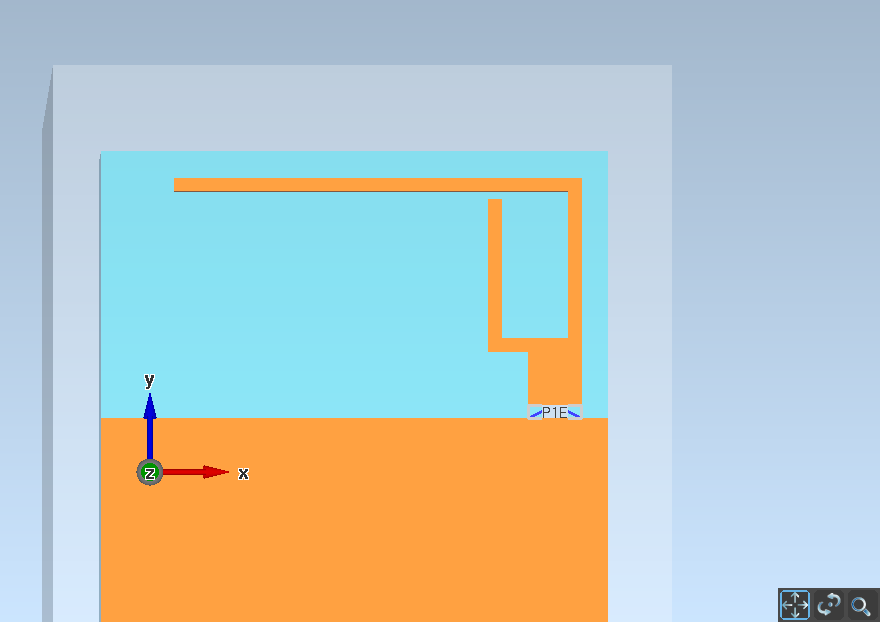
\includegraphics[width=0.7\textwidth]{../fig/plt/crazy_stuff_l4_pcb_v2c_laptop_1a_105_5ghz_3d_pcb_xy.png}
	\caption[Leiterplattenmodell des Antennenentwurfs im Empire.]{
		Leiterplattenmodell des Antennenentwurfs im Empire.
		Die Abbildung zeigt den Antennenbereich der Leiterplatte
		mit der Groundplane (unten), der Antenne (oben) und der
		idealen Einspeisung (zwischen Groundplane und Antenne).
		Hierbei ist das Substrat (FR4) blau dargestellt und das
		Kupfer orange. Die dargestellte Ansicht zeigt das
		Design in der XY Ebene (siehe Koordinatenkreuz).}	
	\label{fig:modell}
\end{figure}

